\documentclass[a4paper,11pt]{article}

\usepackage[french]{babel}
\usepackage[utf8]{inputenc}
\usepackage[left=2.5cm,top=2cm,right=2.5cm,nohead,nofoot]{geometry}
\usepackage{url}
\usepackage{graphicx}
\usepackage{hyperref}
\usepackage{listings}
\usepackage{amsmath}
\usepackage{amssymb}
\usepackage{color}
\usepackage{listings}
\usepackage{graphicx}
\usepackage{float}
\usepackage{todonotes}




\linespread{1.1}



\begin{document}

\begin{titlepage}
\begin{center}
\textbf{\textsc{UNIVERSIT\'E LIBRE DE BRUXELLES}}\\
%\textbf{\textsc{Faculté des Sciences}}\\
%\textbf{\textsc{Département d'Informatique}}
\vfill{}\vfill{}
\begin{center}{\Huge Projet : Logique Propositionnelle et Utilisation de l’Outil MiniSat}\end{center}{\Huge \par}
\begin{center}{\large Pierre Gérard, Antoine Carpentier}\end{center}{\Huge \par}
\vfill{}\vfill{} \vfill{}
\begin{flushleft}{\large \textbf{INFO-F-302 Informatique Fondamentale}}\hfill{Emmanuel FILIOT, Guillermo Pérez}\end{flushleft}{\large\par}
\vfill{}\vfill{}\enlargethispage{3cm}
\textbf{Année académique 2014~-~2015}
\end{center}
\end{titlepage}

%\begin{abstract}
%Ce rapport présente ...
%\end{abstract}


\tableofcontents

\pagebreak


\section{Q1}
Les contraintes sont les suivantes :
\begin{itemize}
  \item Contrainte d'existence : chaque examen se déroule dans au moins une salle et durant au moins une période de temps,
  \item Le nombre d'étudiant dans une salle ne peut pas dépasser sa capacité,
  \item Un étudiant ne peut pas avoir deux examens au même moment,
  \item Un professeur ne peut pas avoir deux examens au même moment,
  \item Un examen doit avoir au moins un professeur,
  \item Un examen doit avoir au moins un étudiant
  \item Chaque examen doit se dérouler exactement une seule fois,
  \item Chaque examen doit se dérouler exactement dans une seule salle,
  \item Dans une salle, il ne peut se déroule qu'un seul examen a la fois.
\end{itemize}


\section{Q2}
\subsection{Contrainte d'existence : chaque examen se déroule dans au moins une salle et durant au moins une période de temps}
\begin{displaymath}
	\forall x \in X, \exists s \in S, \exists t \in T : \mu(x) = (s,t) 
\end{displaymath}

\subsection {Le nombre d'étudiant dans une salle ne peut pas dépasser sa capacité}
\begin{displaymath}
\forall x \in X , \forall s \in S ,\forall e \in E, \forall t \in \{1,...,T\} : a(e) \mapsto \{x\} \wedge \mu(x) = (s,t) \wedge \sum a(e) \mapsto \{x\} \leq c(s)
\end{displaymath}	

\subsection {Un étudiant ne peut pas avoir deux examens au même moment}
\begin{displaymath}
\forall x_{1},x_{2} \in X, \forall s_{1},s_{2} \in S , \forall e \in E ,\forall t_{1}, t_{2} \in \{1,...,T\} :  a(e) \mapsto \{x_{1},x_{2}\}  \wedge \mu(x_{1}) = (s_{1},t_{1}) \wedge \mu(x_{2}) = (s_{2},t_{2}) \wedge t_{1} != t_{2} \wedge x_{1} != x_{2}
\end{displaymath}
\subsection {Un professeur ne peut pas avoir deux examens au même moment}
\begin{displaymath}
\forall x_{1},x_{2} \in X, \forall s_{1},s_{2} \in S , \forall p \in P ,\forall t_{1}, t_{2} \in \{1,...,T\} :  b(p) \mapsto \{x_{1},x_{2}\}  \wedge \mu(x_{1}) = (s_{1},t_{1}) \wedge \mu(x_{2}) = (s_{2},t_{2}) \wedge t_{1} != t_{2} \wedge x_{1} != x_{2}
\end{displaymath}
\subsection {Un examen doit avoir au moins un professeur}
\begin{displaymath}
\forall x \in X, \exists p \in P : b(p) \mapsto \{x\} 
\end{displaymath}
\subsection {Un examen doit avoir au moins un étudiant}
\begin{displaymath}
\forall x \in X, \exists e \in E : a(e) \mapsto \{x\}
\end{displaymath}
\subsection {Chaque examen doit se dérouler une seule fois}
\begin{displaymath}
\forall t_{1}, t_{2} \in \{1,...,T\},\forall s_{1},s_{2} \in S, \nexists x \in X : t_{1} != t_{2} \wedge \mu(x) = (s_{1},t_{1}) \wedge \mu(x) = (s_{2},t_{2})
\end{displaymath}
\subsection {Chaque examen doit se dérouler dans une seule salle}
\begin{displaymath}
\forall t_{1}, t_{2} \in \{1,...,T\},\forall s_{1},s_{2} \in S, \nexists x \in X : s_{1} != s_{2} \wedge \mu(x) = (s_{1},t_{1}) \wedge \mu(x) = (s_{2},t_{2})
\end{displaymath}	
\subsection {Dans une salle, il ne peut se dérouler qu'un seul examen a la fois}
\begin{displaymath}
\forall t_{1}, t_{2} \in \{1,...,T\},\forall x_{1},x_{2} \in X, \nexists s \in S : t_{1} = t_{2} \wedge x_{1} != x_{2} \wedge \mu(x_{1}) = (s,t_{1}) \wedge \mu(x_{2}) = (s,t_{2})
\end{displaymath}	

\section{Q3}
Pour construire la formule en FNC, nous avons besoins de définir de nouvelle variable.
\begin{itemize}
    \item \(E\) est le nombre d'étudiants
    \item \(P\) est le nombre de professeurs
    \item \(X\) est le nombre d'examens
    \item \(S\) est le nombre de salles
    \item \(T\) est le nombre de périodes de temps
	\item \( A_{e,x}\) telle que l'étudiant e passe l'examen x,
	\item \(B_{p,x}\) telle que le professeur p donne l'examen x ,
	\item \(C_{s,i}\) telle que la salle s a la capacité d'accueillir i étudiants,
	\item \(N_{x}\) telle que la fonction N donne le nombre d'étudiant qui passe l'examen x.
\end{itemize}


\subsection{Ensemble de FNC}
\subsubsection{(p1)}
Contrainte d'existence : chaque examen se déroule dans au moins une salle et durant au moins une période de temps
\begin{displaymath}
	\bigwedge\limits_{x=1}^{X}\bigvee\limits_{s=1}^{S}\bigvee\limits_{t=1}^{T} M_{s,x,t}
\end{displaymath}


\subsubsection{(p2)}
Le nombre d'étudiant dans une salle ne peut pas dépasser sa capacité
\begin{displaymath}
	\bigwedge\limits_{t=1}^{T}\bigwedge\limits_{x=1}^{X}\bigwedge\limits_{\substack{s=1 \\ \neg C_{s,N_{x}}}}^{S}  \neg M_{x,s,t}
\end{displaymath}

\subsubsection{(p3)}
Un étudiant ne peut pas avoir deux examens au même moment
\begin{displaymath}
\bigwedge\limits_{e=1}^{E}\bigwedge\limits_{t=1}^{T}\bigwedge\limits_{s_{1}=1}^{S}\bigwedge\limits_{s_{2}=1}^{S}\bigwedge\limits_{\substack{x1=1 \\ A_{e,x_{1}}}}^{X}\bigwedge\limits_{\substack{x_{2}=x_{1}+1 \\ A_{e,x_{2}}}}^{X} \neg M_{x_{1}, s_{1}, t} \vee \neg M_{x_{2}, s_{2}, t}
\end{displaymath}

\subsubsection{(p4)}
Un professeur ne peut pas avoir deux examens au même moment
\begin{displaymath}
\bigwedge\limits_{p=1}^{P}\bigwedge\limits_{t=1}^{T}\bigwedge\limits_{s_{1}=1}^{S}\bigwedge\limits_{s_{2}=1}^{S}\bigwedge\limits_{\substack{x_{1}=1 \\ B_{p,x_{1}}}}^{X}\bigwedge\limits_{\substack{x_{2}=x_{1}+1 \\ B_{p,x_{2}}}}^{X} \neg M_{x_{1}, s_{1}, t} \vee \neg M_{x_{2}, s_{2}, t}
\end{displaymath}

\subsubsection{(p5)}
Un examen doit avoir au moins un professeur
\begin{displaymath}
\bigwedge\limits_{x=1}^{X}\bigvee\limits_{s=1}^{S}\bigvee\limits_{t=1}^{T}\bigvee\limits_{\substack{p=1 \\ B_{p,x}}}^{P} M_{x, s, t}
\end{displaymath}

\subsubsection{(p6)}
Un examen doit avoir au moins un étudiant
\begin{displaymath}
\bigwedge\limits_{x=1}^{X}\bigvee\limits_{s=1}^{S}\bigvee\limits_{t=1}^{T}\bigvee\limits_{\substack{e=1 \\ A_{e,x}}}^{E} M_{x, s, t}
\end{displaymath}

\subsubsection{(p7)}
Chaque examen doit se dérouler une seule fois
\begin{displaymath}
\bigwedge\limits_{x=1}^{X}\bigwedge\limits_{s=1}^{S}\bigwedge\limits_{t_{1}=1}^{T}\bigwedge\limits_{t_{2}=t_{1}+1}^{T} \neg M_{x, s, t_{1}} \vee \neg M_{x, s, t_{2}}
\end{displaymath}

\subsubsection{(p8)}
Chaque examen doit se dérouler dans une seule salle
\begin{displaymath}
\bigwedge\limits_{x=1}^{X}\bigwedge\limits_{t=1}^{T}\bigwedge\limits_{s_{1}=1}^{S}\bigwedge\limits_{s_{2}=t1+1}^{S} \neg M_{x, s_{1}, t} \vee \neg M_{x, s_{2}, t}
\end{displaymath}

\subsubsection{(p9)}
Dans une salle, il ne peut se déroule qu'un seul examen a la fois.
\begin{displaymath}
\bigwedge\limits_{s=1}^{S}\bigwedge\limits_{t=1}^{T}\bigwedge\limits_{x_{1}=1}^{X}\bigwedge\limits_{x_{2}=t1+1}^{X} \neg M_{x_{1}, s, t} \vee \neg M_{x_{2}, s, t}
\end{displaymath}


\subsection{FNC final}
La forme normal conjonctive de la formule est:
\begin{displaymath}
\Phi_{I} = p1 \wedge p2 \wedge p3 \wedge p4 \wedge p5 \wedge p6 \wedge p7 \wedge p8 \wedge p9
\end{displaymath}

\section{Q4}
\subsection{Tester l'implémentation}
Pour tester l'implémentation, utilisez le script bash disponible de la manière suivante :
\begin{lstlisting}
$ sh TestMe.sh	
\end{lstlisting}
Ce script va faire le build, lire les fichiers, et exécuter mini-sate.

\subsection{Parser}
Pour le parser, nous avons décidé de ne pas utiliser l'ensemble du code du parser fournit. Nous avons donc seulement gardé la classe ShedSpec en créant nous même la structure de donnée nécessaire pour son constructeur.

\subsection{Exemple de résultat}
Nous avons créé une liste d'input possible pour cette question. Voici quelque exemple
\subsubsection{Construction d'un horaire possible}
Input fournis avec l'énoncé.
\begin{lstlisting}[
    basicstyle=\tiny, %or \small or \footnotesize etc.
]
$ ./projq4.out "4 ;3 ;10 ;30 ;100 ;100 ;2 ;4 ;1; 1; 1 ;1 ;1 ;1 ;1 ;1 ;1 ;1 ;1 ;1 ;1 ;1 ;1 ;1 ;1 ;1 ;1 ;1
 ;1 ;1 ;1 ;1 ;1 ;1 ;1 ;1 ;1 ;1 ;2 ;2 ;2 ;2 ;2 ;2 ;2 ;2 ;2 ;2 ;2 ;2 ;2 ;2 ;2 ;2 ;2 ;2 ;2 ;2 ;2 ;2 ;2 ;2 
 ;2 ;2 ;2 ;2 ;2 ;2 ;3,4 ;3,4 ;3,4 ;3,4 ;3,4 ;3,4 ;3,4 ;3,4 ;3,4 ;3,4 ;3,4 ;3,4 ;3,4 ;3,4 ;3,4 ;3,4 
 ;3,4 ;3,4 ;3,4 ;3,4 ;3,4 ;3,4 ;3,4 ;3,4 ;3,4 ;3,4 ;3,4 ;3,4 ;3,4 ;3,4 ;3,4 ;3,4 ;3,4 ;3,4 ;3,4 ;3,4 
 ;3,4 ;3,4 ;3,4 ;3,4 ;1,3 ;2,4;
---------------------------------------- Result ----------------------------------------
T = 4
|S| = 3
c(s1) = 10
c(s2) = 30
c(s3) = 100
|E| = 100
|P| = 2
|X| = 4
a(e1) = { 1 }
[...]
a(e30) = { 1 }
[...]
a(e60) = { 2 }
a(e61) = { 3 4 }
[...]
a(e99) = { 3 4 }
a(e100) = { 3 4 }
b(p1) = { 1 3 }
b(p2) = { 2 4 }
==================================[MINISAT]===================================
| Conflicts |     ORIGINAL     |              LEARNT              | Progress |
|           | Clauses Literals |   Limit Clauses Literals  Lit/Cl |          |
==============================================================================
|         0 |     260     3528 |      86       0        0     nan |  0.000 % |
==============================================================================
Success, the problem has been solve under those constraints !
Examen 1 dans la salle 2 au temps 1
Examen 2 dans la salle 2 au temps 2
Examen 3 dans la salle 3 au temps 2
Examen 4 dans la salle 3 au temps 1

OUTPUT : 2,1;2,2;3,2;3,1;
\end{lstlisting}

\subsubsection{Construction d'un horaire impossible}
Input créé de tel manière qu'il n'y ait pas moyen de construire un horaire.
\begin{lstlisting}[
    basicstyle=\tiny, %or \small or \footnotesize etc.
]
$ ./projq4.out "1 ;3 ;1 ;10 ;50 ;2 ;2 ;2 ;1,2 ;1 ;1 ;2 ;"
---------------------------------------- Result ----------------------------------------
T = 1
|S| = 3
c(s1) = 1
c(s2) = 10
c(s3) = 50
|E| = 2
|P| = 2
|X| = 2
a(e1) = { 1 2 }
a(e2) = { 1 }
b(p1) = { 1 }
b(p2) = { 2 }
==================================[MINISAT]===================================
| Conflicts |     ORIGINAL     |              LEARNT              | Progress |
|           | Clauses Literals |   Limit Clauses Literals  Lit/Cl |          |
==============================================================================
|         0 |      18       53 |       6       0        0     nan |  0.000 % |
==============================================================================
Uh .. The problem could not be solve under those constraints

OUTPUT : 0
\end{lstlisting}

\subsection{Nouvelle variable}

\section{Q5}
Pour construire la formule en FNC, nous avons besoins de définir une nouvelle variable :  
\begin{itemize}
	\item \( D_{x}\) qui donne la durée de l'examen x.
\end{itemize}

\subsection{Modification de contrainte}

\subsubsection{Un étudiant ne peut pas avoir deux examens au même moment}
(p3)
\begin{displaymath}
\bigwedge\limits_{e=1}^{E}\bigwedge\limits_{t1=1}^{T}\bigwedge\limits_{\substack{t2=1 \\ t1 <= t2 + D(x2)-1 \wedge t1 + D(x1)-1 >= t2}}^{T}\bigwedge\limits_{s=1}^{S}\bigwedge\limits_{\substack{x1=1 \\ A_{e,x1}}}^{X}\bigwedge\limits_{\substack{x2=x1+1 \\ A_{e,x2}}}^{X} \neg M_{x1, s1, t} \vee \neg M_{x2, s2, t}
\end{displaymath}

\subsubsection{Un professeur ne peut pas avoir deux examens au même moment}
(p4)
\begin{displaymath}
\bigwedge\limits_{p=1}^{P}\bigwedge\limits_{t1=1}^{T}\bigwedge\limits_{\substack{t2=1 \\ t1 <= t2 + D(x2)-1 \wedge t1 + D(x1)-1 >= t2}}^{S}\bigwedge\limits_{s=1}^{S}\bigwedge\limits_{\substack{x1=1 \\ B_{p,x1}}}^{X}\bigwedge\limits_{\substack{x2=x1+1 \\ B_{p,x2}}}^{X} \neg M_{x1, s1, t} \vee \neg M_{x2, s2, t}
\end{displaymath}

\subsubsection{Chaque examen doit se dérouler une seule fois}
(p7)
\begin{displaymath}
\bigwedge\limits_{x=1}^{X}\bigwedge\limits_{s=1}^{S}\bigwedge\limits_{t=1}^{T} \neg M_{x, s, t}
\end{displaymath}


\subsection{Nouvelle contrainte}
\subsubsection{Chaque examen doit avoir un nombre de période de de temps égal à sa durée et ses périodes de temps doivent être continues}

(p10)
\begin{displaymath}
\bigwedge\limits_{x_{1}=1}^{X}\bigwedge\limits_{\substack{x_{2}=1 \\ x_{1} != x_{2}}}^{X}\bigwedge\limits_{s=1}^{S}\bigwedge\limits_{t_{1}=1}^{T}\bigvee\limits_{\substack{t_{2}=0 \\ t_{1} < t_{2} + D(x_{2})-1 \wedge t_{1} + D(x_{1})-1 > t_{2}}}^{T} \neg M_{x_{1}, s, t_{1}} \vee \neg M_{x_{2}, s, t_{2}}
\end{displaymath}

\subsection{FNC}

\begin{displaymath}
	\Phi_{D} = p1 \wedge p2 \wedge p3 \wedge p4 \wedge p5 \wedge p6 \wedge p8 \wedge p9 \wedge p10
\end{displaymath}

\subsection{Exemple de résultats}

\begin{lstlisting}[
    basicstyle=\tiny, %or \small or \footnotesize etc.
]
$ ./projq5.out "12 ;3 ;10 ;30 ;100 ;100 ;2 ;4 ;1; 1; 1 ;1 ;1 ;1 ;1 ;1 ;1 ;1 ;1 ;1 ;1 ;1 ;1 ;1 ;1 ;1 ;
1 ;1 ;1 ;1 ;1 ;1 ;1 ;1 ;1 ;1 ;1 ;1 ;2 ;2 ;2 ;2 ;2 ;2 ;2 ;2 ;2 ;2 ;2 ;2 ;2 ;2 ;2 ;2 ;2 ;2 ;2 ;2 ;2 ;2 ;
2 ;2 ;2 ;2 ;2 ;2 ;2 ;2 ;3,4 ;3,4 ;3,4 ;3,4 ;3,4 ;3,4 ;3,4 ;3,4 ;3,4 ;3,4 ;3,4 ;3,4 ;3,4 ;3,4 ;3,4 ;
3,4 ;3,4 ;3,4 ;3,4 ;3,4 ;3,4 ;3,4 ;
3,4 ;3,4 ;3,4 ;3,4 ;3,4 ;3,4 ;3,4 ;3,4 ;3,4 ;3,4 ;3,4 ;3,4 ;3,4 ;3,4 ;3,4 ;3,4 ;3,4 ;3,4 ;1,3 ;
2,4; 2; 4; 2; 3;"

---------------------------------------- Result ----------------------------------------
T = 12
|S| = 3
c(s1) = 10
c(s2) = 30
c(s3) = 100
|E| = 100
|P| = 2
|X| = 4
a(e1) = { 1 }
[...]
a(e30) = { 1 }
a(e31) = { 2 }
[...]
a(e60) = { 2 }
a(e61) = { 3 4 }
[...}
a(e99) = { 3 4 }
a(e100) = { 3 4 }
b(p1) = { 1 3 }
b(p2) = { 2 4 }
d(x1) = 2
d(x2) = 4
d(x3) = 2
d(x4) = 3
==================================[MINISAT]===================================
| Conflicts |     ORIGINAL     |              LEARNT              | Progress |
|           | Clauses Literals |   Limit Clauses Literals  Lit/Cl |          |
==============================================================================
|         0 |    1868    36217 |     622       0        0     nan |  0.000 % |
==============================================================================
Success, the problem has been solve under those constraints !
Examen 1 dans la salle 2 au temps 1
Examen 2 dans la salle 2 au temps 4
Examen 3 dans la salle 3 au temps 4
Examen 4 dans la salle 3 au temps 1

OUTPUT : 2,1;2,4;3,4;3,1;

\end{lstlisting}


\section{Q6}

\subsection{Hypothèse}
Pour cette question, nous avons supposé que les examens se déroulaient tous les jours de 8h à 20h. L'ensemble de paires tels que ont ne pas pas avoir d'examen ont été codés dans la classe SchedSpec sous la variable I. Notre implémentation permet de les modifiers sans avoir à modifier le reste du code.

\todo{Verifier que c'est bien de 8h a 20h}

\subsection{Nouvelle variable}

Pour construire la formule en FNC, nous avons besoins de définir une nouvelle variable :  
\begin{itemize}
	\item \( J_{t}\) tel que t fait partit du jour, c'est à dire qu'il est possible d'avoir un examen en t.
\end{itemize}

\subsection{Modification de contrainte}
Aucune contrainte déjà existante n'a du être modifié pour ce problème.

\subsection{Nouvelle contrainte}
\subsubsection{Aucun examen ne peut se dérouler durant les intervals défini par I.} \todo{Meilleur description de la contrainte}
(p11)
\begin{displaymath}
\bigwedge\limits_{x_{1}=1}^{X}\bigwedge\limits_{s=1}^{S}\bigwedge\limits_{\substack{t=0 \\ \neg J(t) }}^{T} \neg M_{x, s, t}
\end{displaymath}

\subsection{FNC}
\begin{displaymath}
	\Phi_{N} = p1 \wedge p2 \wedge p3 \wedge p4 \wedge p5 \wedge p6 \wedge p8 \wedge p9 \wedge p10 \wedge p11
\end{displaymath}
\subsection{Exemple de résultats}
20 examens, durée variant de 1 à 4 et 1 à 4 examen par étudiant.

\begin{lstlisting}[
    basicstyle=\tiny, %or \small or \footnotesize etc.
]
$ ./projq6.out "100;10;100;150;147;49;154;174;62;164;121;181;100;10;20;20,7,19;17,7,2;10,11,15;13,4,19;6,9,11;
17,8,5;17,8,16;20,2,1;15,11,6;4,4,19;11,10,9;6,13,16;3,17,10;2,6,11;16,19,12;5,13,9;20,11,15;7,9,13;
14,2,3;5,15,11;2,2,16;14,10,18;16,4,1;6,19,4;6,19,7;11,11,20;16,15,20;14,20,8;13,20,9;8,6,6;4,17,7;
15,3,16;17,15,19;10,10,4;7,14,9;10,6,6;4,11,1;15,3,2;16,9,8;18,5,11;6,18,20;13,13,3;1,10,1;15,6,19;
3,1,15;10,2,6;7,19,11;13,18,18;4,19,1;17,12,1;9,5,8;11,16,1;19,12,4;2,8,2;6,14,6;10,13,6;11,14,10;
9,17,19;6,2,2;9,5,11;10,11,8;20,13,3;11,1,6;13,4,9;12,6,12;7,5,13;15,7,2;17,18,13;13,8,9;7,16,3;
18,2,17;4,13,19;5,15,6;3,19,7;10,15,13;19,18,6;9,9,10;20,14,9;20,19,20;17,4,1;4,12,18;17,11,15;
13,8,15;5,3,20;12,15,7;9,2,15;3,11,16;1,7,2;6,14,1;8,9,20;19,9,16;12,16,16;5,15,9;20,19,16;4,20,20;
3,1,18;3,18,8;17,1,9;14,13,13;6,1,13;2,7,3,16,1;12,11,15,13,18;5,8,2;6,6,19,20,10;5;14,1,20,5;
4,4,5,7,8;6,15,10,17,9;1,9;20,16,2,1;4;1;1;4;4;1;1;4;1;4;1;4;2;2;4;3;2;3;3;3;"

==================================[MINISAT]===================================
| Conflicts |     ORIGINAL     |              LEARNT              | Progress |
|           | Clauses Literals |   Limit Clauses Literals  Lit/Cl |          |
==============================================================================
|         0 | 6020540 12069760 | 2006846       0        0    -nan |  0.000 % |
==============================================================================
Success, the problem has been solve under those constraints !
Examen 1 dans la salle 1 au temps 81
Examen 2 dans la salle 1 au temps 14
Examen 3 dans la salle 1 au temps 42
Examen 4 dans la salle 1 au temps 67
Examen 5 dans la salle 1 au temps 63
Examen 6 dans la salle 1 au temps 62
Examen 7 dans la salle 1 au temps 61
Examen 8 dans la salle 1 au temps 57
Examen 9 dans la salle 1 au temps 17
Examen 10 dans la salle 1 au temps 44
Examen 11 dans la salle 1 au temps 43
Examen 12 dans la salle 1 au temps 39
Examen 13 dans la salle 1 au temps 37
Examen 14 dans la salle 1 au temps 19
Examen 15 dans la salle 1 au temps 33
Examen 16 dans la salle 1 au temps 20
Examen 17 dans la salle 1 au temps 18
Examen 18 dans la salle 1 au temps 15
Examen 19 dans la salle 1 au temps 12
Examen 20 dans la salle 1 au temps 9
 
OUTPUT : 1,81;1,14;1,42;1,67;1,63;1,62;1,61;1,57;1,17;1,44;1,43;1,39;1,37;1,19;1,33;1,20;1,18;1,15;1,12;1,9;


\end{lstlisting}
\section{Q7}
\subsection{Nouvelle contrainte}
\subsubsection{La somme, pour tout étudiant e, du nombre de changements de salle de e, est bornée par k}
(p12)
\begin{displaymath}
	TODO	
\end{displaymath}

\subsection{FNC}
\begin{displaymath}
	\Phi_{N} = p1 \wedge p2 \wedge p3 \wedge p4 \wedge p5 \wedge p6 \wedge p8 \wedge p9 \wedge p10 \wedge p11 \wedge p12
\end{displaymath}
	
\subsection{Implémentation}
\subsection{Exemple de résultats}

\section{Q8}

\section{Q9}

\subsection{Modification de contrainte}
\subsubsection{Un étudiant ne peut pas avoir deux examens au même moment}
(p3a)
\begin{displaymath}
\bigwedge\limits_{e=1}^{E}\bigwedge\limits_{t1=1}^{T}\bigwedge\limits_{\substack{t2=1 \\ t1 <= t2 + D(x2) \wedge t1 + D(x1) >= t2}}^{T}\bigwedge\limits_{s_{1}=1}^{S}\bigwedge\limits_{\substack{s2=1 \\ s_{1} != s_{2}}}^{S}\bigwedge\limits_{\substack{x1=1 \\ A_{e,x1}}}^{X}\bigwedge\limits_{\substack{x2=x1+1 \\ A_{e,x2}}}^{X} \neg M_{x1, s1, t} \vee \neg M_{x2, s2, t}
\end{displaymath}
(p3b)
\begin{displaymath}
\bigwedge\limits_{e=1}^{E}\bigwedge\limits_{t1=1}^{T}\bigwedge\limits_{\substack{t2=1 \\ t1 <= t2 + D(x2)-1 \wedge t1 + D(x1)-1 >= t2}}^{T}\bigwedge\limits_{s_{1}=1}^{S}\bigwedge\limits_{\substack{s2=1 \\ s_{1} = s_{2}}}^{S}\bigwedge\limits_{\substack{x1=1 \\ A_{e,x1}}}^{X}\bigwedge\limits_{\substack{x2=x1+1 \\ A_{e,x2}}}^{X} \neg M_{x1, s1, t} \vee \neg M_{x2, s2, t}
\end{displaymath}

$ (p3) = (p3a) \wedge (p3b) $
\subsection{FNC}
\begin{displaymath}
	\Phi_{N} = p1 \wedge p2 \wedge p3 \wedge p4 \wedge p5 \wedge p6 \wedge p8 \wedge p9 \wedge p10 \wedge p11 \wedge p12
\end{displaymath}
\subsection{Implémentation}
\subsection{Exemple de résultats}

\section{Q10}
\subsection{Certains examens dans certaines salles (ex. salle informatique)}
Pour modéliser la contrainte, nous avons besoins de définir une nouvelle variable :  
\begin{itemize}
	\item \( XS_{x,s}\) tel que l'examen x peut se dérouler dans la salle s.
\end{itemize}
\begin{displaymath}
	\bigwedge\limits_{x=1}^{X}\bigwedge\limits_{\substack{s=1 \\ \neg XS(x,s)}}^{S}\bigwedge\limits_{t=1}^{T} \neg M_{x, s, t} 
\end{displaymath}


\subsection{Si deux examens se suivent et sont sur des campus différents, il y a 2 temps entre ces deux examens}
Faisons les hypothèses suivantes : 
Pour modéliser la contrainte, nous avons besoins de définir une nouvelle variable :  
\begin{itemize}
	\item \( SC_{s1,s2}\) tel que s1 est sur un campus différent de s2.
\end{itemize}
Pou réaliser cela, nous devons modifier la contrainte p3: \todo{Nom de la contrainte}

(p3a) Pas de changement de salle
\begin{displaymath}
\bigwedge\limits_{e=1}^{E}\bigwedge\limits_{t1=1}^{T}\bigwedge\limits_{\substack{t2=1 \\ t1 <= t2 + D(x2)-1 \wedge t1 + D(x1)-1 >= t2}}^{T}\bigwedge\limits_{s_{1}=1}^{S}\bigwedge\limits_{\substack{s2=1 \\ s_{1} = s_{2}}}^{S}\bigwedge\limits_{\substack{x1=1 \\ A_{e,x1}}}^{X}\bigwedge\limits_{\substack{x2=x1+1 \\ A_{e,x2}}}^{!X} \neg M_{x1, s1, t} \vee \neg M_{x2, s2, t}
\end{displaymath}

(p3b) Changement de salle et de campus
\begin{displaymath}
\bigwedge\limits_{e=1}^{E}\bigwedge\limits_{t1=1}^{T}\bigwedge\limits_{\substack{t2=1 \\ t1 <= t2 + D(x2) +1 \wedge t1 + D(x1) +1 >= t2}}^{T}\bigwedge\limits_{s_{1}=1}^{S}\bigwedge\limits_{\substack{s2=1 \\ s_{1} != s_{2} \wedge SC_{s1,s2}}}^{S}\bigwedge\limits_{\substack{x1=1 \\ A_{e,x1}}}^{X}\bigwedge\limits_{\substack{x2=x1+1 \\ A_{e,x2}}}^{X} \neg M_{x1, s1, t} \vee \neg M_{x2, s2, t}
\end{displaymath}

(p3c) Changement de salle mais pas de campus
\begin{displaymath}
\bigwedge\limits_{e=1}^{E}\bigwedge\limits_{t1=1}^{T}\bigwedge\limits_{\substack{t2=1 \\ t1 <= t2 + D(x2) \wedge t1 + D(x1) >= t2}}^{T}\bigwedge\limits_{s_{1}=1}^{S}\bigwedge\limits_{\substack{s2=1 \\ s_{1} != s_{2} \wedge \neg SC_{s1,s2} }}^{S}\bigwedge\limits_{\substack{x1=1 \\ A_{e,x1}}}^{X}\bigwedge\limits_{\substack{x2=x1+1 \\ A_{e,x2}}}^{X} \neg M_{x1, s1, t} \vee \neg M_{x2, s2, t}
\end{displaymath}


$ (p3) = (p3a) \wedge (p3b) \wedge (p3c)$


\section{Q11}
Pour rappel, voici les différentes complexités P, NP, NP-complet et NP-dur.
\begin{figure}[H]
  \centering
  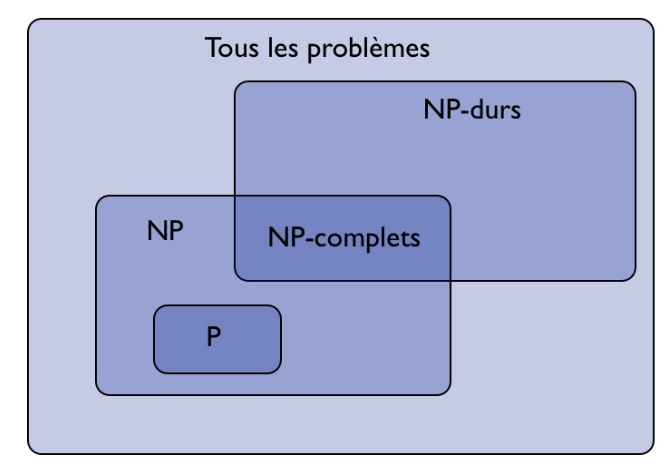
\includegraphics[scale=0.4]{images/q11-p-np-nphardcomplete.png}
  \caption{\label{} P, NP, NP-complet et NP-dur}
\end{figure}
Pour prouver qu'un problème est NP-dur, il faut montrer qu'un problème NP-dur connu peut se ramener à notre problème.

Nous allons donc montrer qu'il existe une bijection entre notre problème d'emploi du temps et le problème de \textbf{Job Shop Scheduling with Sequence-Dependent Setup}. Le problème de Job Shop Scheduling with Sequence-Dependent Setup est NP-dur \footnote{Artigues, Christian, Sana Belmokhtar, and Dominique Feillet. "A new exact solution algorithm for the job shop problem with sequence-dependent setup times." \textit{Integration of ai and or techniques in constraint programming for combinatorial optimization problems}. Springer Berlin Heidelberg, 2004. 37-49.}.

On pose les examens comme étant des jobs, les salles comme étant des machines allouables aux jobs, la durée d'un examen comme étant la durée d'un job et on garde les périodes de temps. Dans une salle (machine), il ne peut pas y avoir deux examens (jobs) en même temps. Chaque examen (job) doit se dérouler exactement une fois et avec exactement une salle (machine).
La capacité des salles dans notre problème peut être modélisée avec la fonction de coût dans le JSS-SDS en donnant un coût infini à un certain examen (job) dans une certaine salle (machine) si le nombre d'étudiants à cette examen excède la capacité de la salle et un coût fini dans le cas contraire.
Les examens que passent un étudiant et ceux que donnent un professeur sont simplement des contraintes externes empêchant certains examens (jobs) de se dérouler en même temps. De même, le fait qu'un examen doit avoir au minimum un étudiant et un professeur est une contrainte externe.
Le but du \textbf{Job Shop Scheduling with Sequence-Dependent Setup} est de minimiser le temps total d'exécution des jobs, ce qui est également le cas avec notre problème puisqu'il faut effectuer tous les examens dans une certaine période de temps T et donc minimiser le temps total.
\end{document}

